\section{Accepttest}
Indgangsimpedansen for alle indgange gav samme målinger, hvilket derfor fører til samme indgangsimpedans for alle udgange. Indgangsimpedansen, for et slukket og et tændt signal, er, som vist i Appendiks \ref{maalejournal_indgangsvaelger}, henholdsvis 22,62 k\ohm~ og 31,56 k \ohm . Da disse begge er over 22 k\ohm~ er indgangsimpedansen acceptabel.

Frekvensgangen for 200 mV og 2 V, er meget éns, derfor tages der kun udgangspunkt i den ene. Det er valgt at konkludere på frekvensgangen for 200 mV, da denne giver det største udsving. En graf over de målte data kan ses på figur \ref{fig:indacc:frek200mv}.
\begin{figure}[h]
\centering
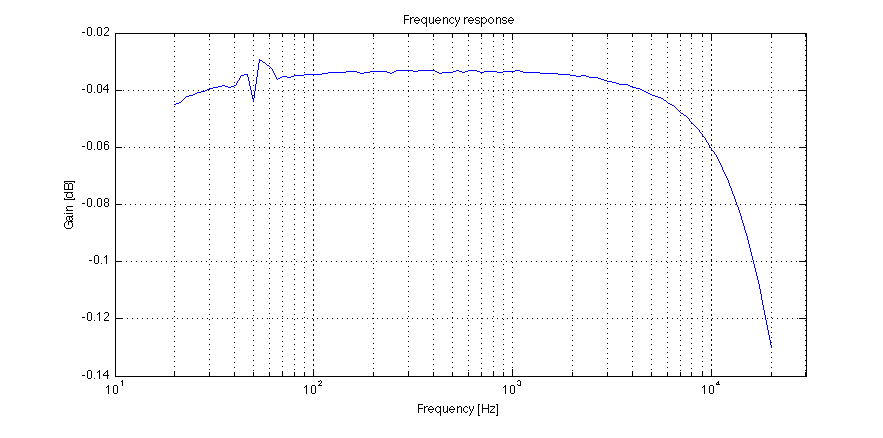
\includegraphics[width=\textwidth]{maalerapporter/indgangsvaelger/Indgangsvlger-mic-200mv-frek.png}
\caption{Målt frekvensgang for mikrofonindgangen på indgangsvælgeren ved 200 mV}
\label{fig:indacc:frek200mv}
\end{figure}

Frekvensgangen for et tændt signal fra 20 Hz til 20 kHz giver signalet måles ud fra en referencefrekvens på 1 kHz. Denne er aflæst til -0,034 dB. Den frekvens som afviger mest fra denne værdi er ved 20 kHz, som aflæses til en dæmpning på -0,13 dB. Dette giver en afvigelse i frekvensgangen på ca. 0,1 dB, hvilket er acceptabelt.

Ved simulering findes dæmpningen, når signalet et slukket, til -94,3 dB, hvilket mere end opfylder kravet. Dette illustreres på figur \ref{fig:indaccept:slukketsimulering}.
\begin{figure}[h]
\centering
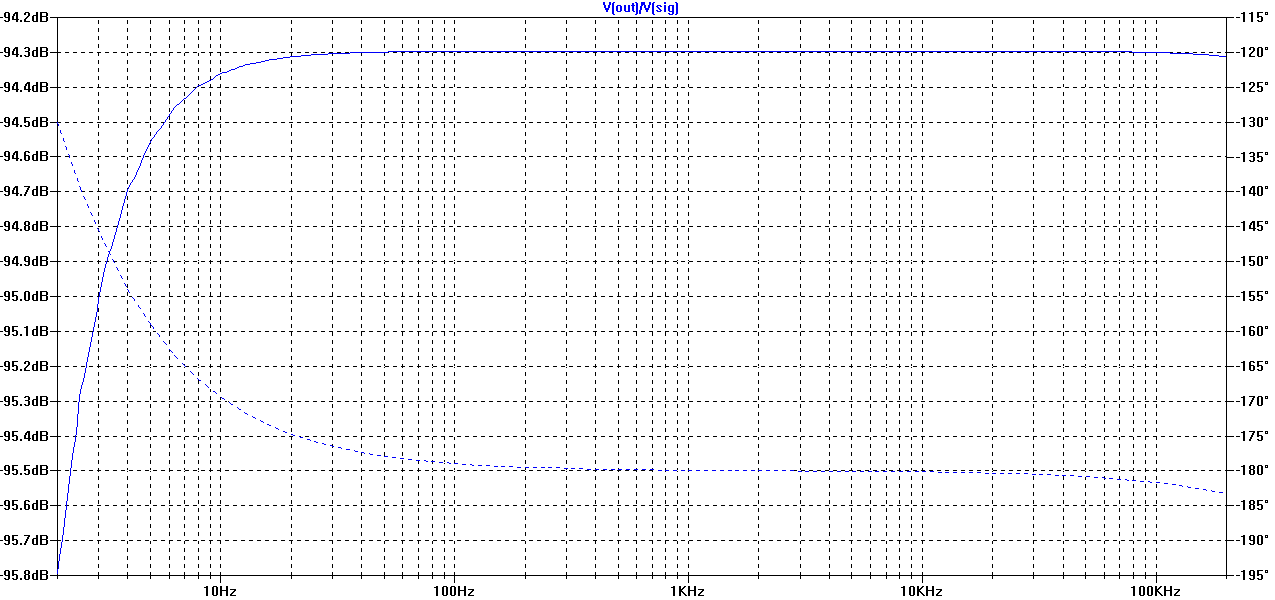
\includegraphics[width=\textwidth]{teknisk/indgangsvaelger/simulering/daempning_af_signal.png}
\caption{Dæmpningsgraden af signalet, når det er slukket.}
\label{fig:indaccept:slukketsimulering}
\end{figure}

Målingerne viser, på figur \ref{fig:indaccept:slukketmaaling}, at dæmpning ved 1 kHz er på ca. -114 dB, hvilket er acceptabelt.
\begin{figure}[h]
\centering
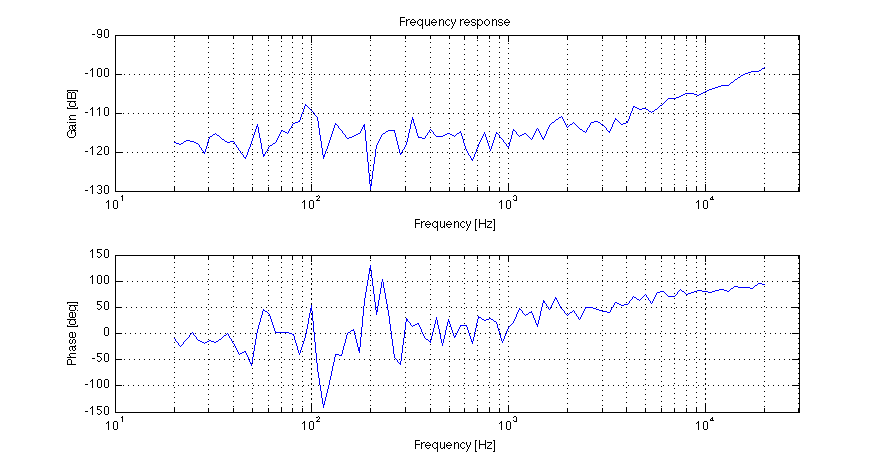
\includegraphics[width=\textwidth]{maalerapporter/indgangsvaelger/Indgangsvlger-mic-2v-slukket-frek.png}
\caption{Frekvensgangen og fasedrejet for mikrofonindgangen for et slukket signal, på indgangsvælgeren ved 2V. Disse målinger er sansynligvis støj, da spændinger på et meget lavt niveau}
\label{fig:indaccept:slukketmaaling}
\end{figure}	

THD simuleres til 0,062\% ved en amplitudespænding på 2 V, ved 1 kHz, se afsnit \ref{indgangsvaelger}. Ved en THD måling, illustreret på figur \ref{fig:accind:thd2v}, aflæses THD'en ved 1kHz til 0,1\%. 
\begin{figure}[h]
\centering
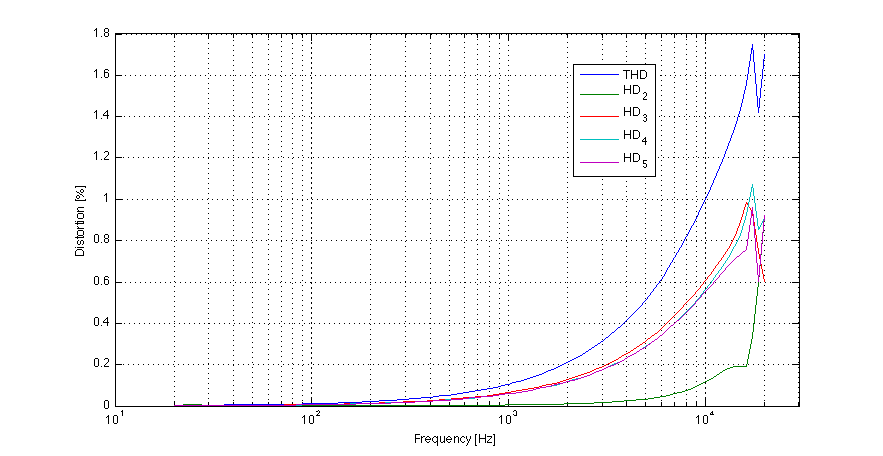
\includegraphics[width=\textwidth]{maalerapporter/indgangsvaelger/Indgangsvlger-mic-2v-thd.png}
\caption{THD for mikrofonindgangen på indgangsvælgeren ved 2 V.}
\label{fig:accind:thd2v}
\end{figure}
Det kan dog konkluderes at THD ikke er lav nok. Dette kan delvist løses ved at benytte en anden operationsforstærker, f.eks. OPA27 i stedet for LM324. Det er dog tydeligt, ud fra appendiks F, at transistorerne ikke afbryder helt, når signalet ikke skal slukkes og at de derfor har en indflydelse. Dette er ikke optimalt og det ville derfor være smart at benytte en transistor, som afkobler bedre i slukket tilstand.